\documentclass[../Main.tex]{subfiles}
\begin{document}
\chapter{Distributed Systems}

\intro{

}

\section{Introduction}

Goals:
\begin{enumerate}
    \item Scaling (one system is not enough)
    \item Location (move systems closer to the consumer)
    \item Fault-Tolerance (Hw will fail eventually)
\end{enumerate}

\defn{Scaling}{
    \begin{description}
        \item[Vertical] Scale systems by adding more resources to already
        existing servers. Is generally cheaper until you max out the hardware.
        No adaption of software required and is thus less complex. THe need of redundancy can pose a problem.
        \item[Horizontal] Add more nodes. In long term massive scaling
        it could be economically more feasable. It adds complexity and needs software adaption.
        The addition of fault tolerance is easier.
    \end{description}
}

\begin{figure}[H]
    \centering
    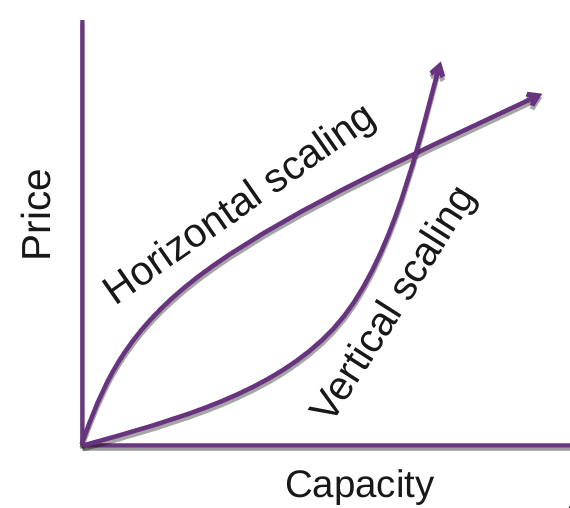
\includegraphics[width=0.25\linewidth]{Images/eco-scaling.png}
    \caption{}
\end{figure}

\defn{Some well known "laws"}{
    Moore's Law:
    \begin{itemize}
        \item The numbers of transistors doubles every 2 years.
    \end{itemize}
    Nielsen's Law:
    \begin{itemize}
        \item A high-end user's connection speed grows by 50\% per year.
    \end{itemize}
    Kryder's Law:
    \begin{itemize}
        \item Disk density douples every 13 months.
    \end{itemize}
    (Kryder's law is not applicable anymore since 2005, because consumer behaviour changed in favor of SSD's)
}

Bandwidth grows slower than compute power. Hence currently it makes sense
to prioritize the optimization of network communication.


\begin{figure}[H]
    \centering
    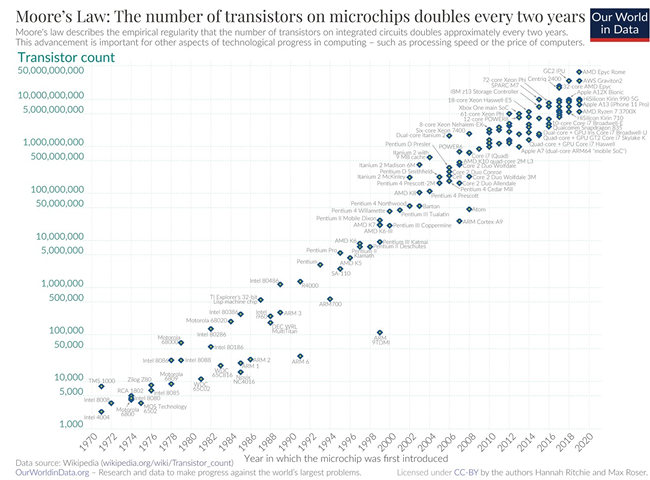
\includegraphics[width=0.5\linewidth]{Images/moore-law.png}
    \caption{Moore's Law}
\end{figure}

\begin{figure}[H]
    \centering
    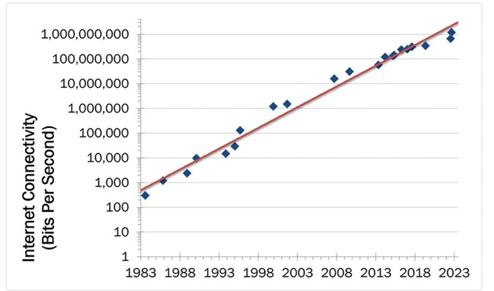
\includegraphics[width=0.5\linewidth]{Images/nielsen-law.png}
    \caption{Nielsen's Law}
\end{figure}

\section{Location}

Why we distribute:
\begin{itemize}
    \item Everything gets faster (CPU, bandwidth, SSD), but latency remains.
    \item Einstein: Nothing in nature is faster than the speed of light $\Rightarrow$ latency is unavoidable.
    \item Speed of light in vacuum: $\approx 300'000$ km/s.
    \item Latency (RTT) is the time for a signal to travel to the destination and back.
    \item Example: Light travel time to Sydney:
    \[
    \left(\frac{16540}{300000}\right) \times 1000 \times 2 \approx 110 \text{ms}, \quad \text{in practice: } \approx 298 \text{ms}.
    \]
    \item Space example: Starlink (LEO $\approx 550$ km)
    \begin{itemize}
        \item Theoretical latency: $7.3$ ms.
        \item Practical latency: $20-60$ ms.
    \end{itemize}
\end{itemize}

\subsection{Light Speed}
Velocity Factos: \href{https://en.wikipedia.org/wiki/Velocity_factor}{Velocity Factors}
\begin{itemize}
    \item \textbf{Latency Discrepancies:}
    \begin{itemize}
        \item \textbf{Sydney Example:} Theoretical RTT: 110\,ms; Practical RTT: 298\,ms.
        \item \textbf{Starlink Example:} Theoretical RTT: 7.3\,ms; Practical RTT: 20--60\,ms.
    \end{itemize}
    \item \textbf{Contributing Factors:}
    \begin{itemize}
        \item \textbf{Indirect Paths:}
        \begin{itemize}
            \item Land route in Europe (Switzerland to Mediterranean coast): $\sim$1,000\,km.
            \item Possible SeaMeWe-5 route: $\sim$16,000\,km.
            \item Singapore to Sydney (undersea cable): $\sim$7,000\,km.
            \item Total estimated distance: $\sim$24,000\,km.
            \item Estimated RTT: 
            \[
            \left(\frac{24,000\,\text{km}}{300,000\,\text{km/s}}\right) \times 2 \times 1,000\,\text{ms/s} = 160\,\text{ms}
            \]
            \item Still less than the observed 298\,ms.
        \end{itemize}
        \item \textbf{Signal Propagation Speed:}
        \begin{itemize}
            \item Speed of light in vacuum: $\sim$300,000\,km/s.
            \item Speed in optical fiber: $\sim$200,000\,km/s.
            \item \textbf{Reference:} \href{https://en.wikipedia.org/wiki/Optical_fiber}{Optical Fiber - Wikipedia}
        \end{itemize}
        \item \textbf{Fiber Types and Materials:}
        \begin{itemize}
            \item Single-mode fibers offer lower latency than multimode fibers due to differences in refractive index and light wavelength.
            \item Hollow-core fibers can further reduce latency.
            \item \textbf{Reference:} \href{https://www.ft.com/content/4307c389-f8b1-42f4-9623-256264b2c611}{Cailabs and Hollow-Core Fiber Technology}
        \end{itemize}
    \end{itemize}
\end{itemize}

Submarine Cable Map: \href{https://www.submarinecablemap.com/submarine-cable/apollo}{Sumbarine Cable Map}

\begin{itemize}
    \item \textbf{Theoretical vs. Practical Latency:}
    \begin{itemize}
        \item \textbf{Fiber Optic Example:}
        \begin{itemize}
            \item Estimated distance: 24,000\,km.
            \item Speed of light in fiber: $\sim$200,000\,km/s.
            \item Theoretical RTT:
            \[
            \left(\frac{24,000\,\text{km}}{200,000\,\text{km/s}}\right) \times 2 \times 1,000\,\text{ms/s} = 240\,\text{ms}
            \]
            \item Observed RTT: $\sim$298\,ms.
        \end{itemize}
        \item \textbf{Contributing Factors to Increased Latency:}
        \begin{itemize}
            \item Non-optimal routing.
            \item Queuing and routing delays.
            \item Traffic inspection.
            \item Signal repeating.
            \item Protocol overhead.
            \item Additional latency: $\sim$50--60\,ms.
        \end{itemize}
    \end{itemize}
    \item \textbf{Satellite Communication Advantages:}
    \begin{itemize}
        \item Direct connections with minimal interference.
        \item Signal propagation through air/space at nearly 300,000\,km/s.
        \item \textbf{Starlink Example:}
        \begin{itemize}
            \item Satellite altitude: $\sim$1,123\,km.
            \item Theoretical RTT:
            \[
            \left(\frac{2 \times 1,123\,\text{km}}{300,000\,\text{km/s}}\right) \times 2 \times 1,000\,\text{ms/s} \approx 15\,\text{ms}
            \]
            \item Practical RTT: 20--60\,ms.
        \end{itemize}
    \end{itemize}
    \item \textbf{Wi-Fi Latency Considerations:}
    \begin{itemize}
        \item Factors contributing to increased latency:
        \begin{itemize}
            \item Carrier Sense Multiple Access with Collision Avoidance (CSMA/CA).
            \item Wait times before transmission.
            \item Acknowledgment packets and retransmissions.
            \item Signal processing delays at transmitter and receiver.
            \item Medium Access Control (MAC) layer processing.
            \item Protocol stack traversal.
            \item Distributed Coordination Function (DCF) backoff.
            \item Channel busy waiting.
        \end{itemize}
        \item Typical additional latency: +5\,ms.
    \end{itemize}
    \item \textbf{Latency Comparison: Satellites vs. Fiber:}
    \begin{itemize}
        \item \textbf{Satellite (Vacuum):}
        \begin{itemize}
            \item Distance: 2,246\,km (round trip).
            \item Speed of light: 300,000\,km/s.
            \item Theoretical RTT:
            \[
            \left(\frac{2,246\,\text{km}}{300,000\,\text{km/s}}\right) \times 1,000\,\text{ms/s} \approx 15\,\text{ms}
            \]
        \end{itemize}
        \item \textbf{Fiber (Glass):}
        \begin{itemize}
            \item Distance: 1,880\,km.
            \item Speed of light in fiber: 150,000\,km/s.
            \item Theoretical RTT:
            \[
            \left(\frac{1,880\,\text{km}}{150,000\,\text{km/s}}\right) \times 2 \times 1,000\,\text{ms/s} \approx 25\,\text{ms}
            \]
        \end{itemize}
    \end{itemize}
    \item \textbf{Conclusion:}
    \begin{itemize}
        \item Satellites, especially those in low Earth orbit like Starlink, can offer lower latency compared to traditional fiber optics due to shorter signal travel distances and higher propagation speeds.
        \item \textbf{Reference:} \href{https://en.wikipedia.org/wiki/Starlink}{Starlink - Wikipedia}
    \end{itemize}
\end{itemize}

\section*{Copper vs. Fiber Optic Cables}

\begin{itemize}
    \item \textbf{Propagation Speed:}
    \begin{itemize}
        \item Copper cables can have lower latency than fiber optics over short distances (under 10 meters)
        due to faster signal propagation.
        \item The latency differences between fiber and copper are influenced by transmission distance,
        speed, and environments.
    \end{itemize}
    \item \textbf{Latency Variations:}
    \begin{itemize}
        \item Depending on the fiber material, latency can change.
    \end{itemize}
\end{itemize}

\section*{Importance of Latency in Distributed Systems}

\begin{itemize}
    \item \textbf{Impact on E-commerce:}
    \begin{itemize}
        \item Amazon found that every 100\,ms of added latency resulted in a 1\% loss in sales.
    \end{itemize}
    \item \textbf{Impact on Search Engines:}
    \begin{itemize}
        \item Google observed that an extra 500\,ms in search page generation led to a 20\% drop in traffic.
        \item Bing reported that a 500\,ms delay caused a 1.2\% decrease in revenue.
    \end{itemize}
    \item \textbf{Impact on Online Gaming:}
    \begin{itemize}
        \item Online games are sensitive to latency, as fast response times are crucial for optimal performance.
        High latency can result in slow responses, giving players with low-latency connections a technical advantage.
    \end{itemize}
\end{itemize}

\subsection{Measures}
\begin{itemize}
    \item Reduce latency but always keep in mind that no matter what you will always have latency
    \item Put services closer to the user 
    \begin{itemize}
        \item Reduce Latency
        \item Increased bandwidth and throughput
        \item Improved reliability and availability
        \item Communication and coordination overhead of data replication and caching
        \item E.g CDN
    \end{itemize}
\end{itemize}

\section{Fault Tolerance}

Random Bit Flips:
\begin{itemize}
    \item Computers typically experience about one comsic-ray induced error per 256 megabytes of RAM per month
    \item Google Study: more than 8\% if DUNNS affected by errirs oer year
    \item Cosmic rays are always present
\end{itemize}

Contributing Factors:
\begin{itemize}
    \item Sensitivity of transistors
    \item Number of transistors
    \item Altitude
    \item Many more
\end{itemize}

Error Correcting codes:
\begin{itemize}
    \item Can mitigate this thread
    \item TMR or Hamming Code can correct 1 flip and detect 2 flips
    \item Not in mainstream consumer market
\end{itemize}

\subsection{Disk Failures}

\begin{itemize}
    \item \textbf{Mechanical Components:} Hard Disk Drives (HDDs) contain moving parts, such as spinning platters and read/write heads, making them susceptible to mechanical failures over time.
    \item \textbf{Failure Rates:} Studies have shown that actual annualized failure rates (AFRs) for
    HDDs range from 1.7\% in the first year to over 8.6\% by the third year. \cite{turn0search24}
    \item \textbf{S.M.A.R.T. Monitoring:} Self-Monitoring, Analysis, and Reporting Technology (S.M.A.R.T.)
    can help predict potential drive failures by monitoring various parameters, though it may not always provide early warnings. \cite{turn0search24}
\end{itemize}

\begin{itemize}
    \item \textbf{NAND Flash Lifespan:} Solid-State Drives (SSDs) use NAND flash memory cells with a limited number of write/erase cycles:
    \begin{itemize}
        \item \textbf{Single-Level Cell (SLC):} 50,000–100,000 cycles.
        \item \textbf{Multi-Level Cell (MLC):} 5,000–10,000 cycles.
        \item \textbf{Triple-Level Cell (TLC):} Approximately 1,000 cycles.
        \item \textbf{Quad-Level Cell (QLC):} Endurance ratings vary; some sources indicate less than 1,000 cycles,
        while others suggest a range between 100 and 1,500 cycles. \cite{turn0search25}
    \end{itemize}
    \item \textbf{Wear Leveling:} SSDs implement wear leveling algorithms to distribute write and erase operations evenly across memory cells, prolonging the device's lifespan.
    \item \textbf{Over-Provisioning:} Manufacturers allocate extra NAND cells as spares to replace worn-out ones, maintaining storage capacity and performance.
    \item \textbf{Monitoring Tools:} Utilities like \texttt{smartctl -a /dev/xyz} can provide insights into an SSD's health and usage of spare cells.
\end{itemize}

\subsection{Inevitability of Hardware Failures}

\begin{itemize}
    \item \textbf{Memory Errors:} Bit flips in memory can occur due to various factors, including cosmic rays and electrical interference.
    \item \textbf{Storage Wear:} Solid-State Drives (SSDs) have a limited number of write/erase cycles, leading to wear over time.
    \item \textbf{Physical Damage:} Network cables and other hardware components can be damaged physically, affecting system performance.
    \item \textbf{Certainty of Failure:} Hardware components will inevitably fail; it's a matter of "when," not "if."
\end{itemize}

\subsection{Advantages of Distributed Systems}

\begin{itemize}
    \item \textbf{Redundancy:} Multiple machines provide redundancy; if one fails, others can take over.
    \item \textbf{Fault Tolerance:} Systems continue to function despite individual failures, enhancing reliability.
    \item \textbf{Load Redistribution:} Workloads can be redistributed among remaining machines, maintaining performance.
\end{itemize}

\subsection{Considerations in Implementing Distributed Systems}

\begin{itemize}
    \item \textbf{Increased Complexity:} Distributed systems add complexity to system design and maintenance.
    \item \textbf{Cost-Benefit Analysis:} Implement distributed systems only when the benefits outweigh the added complexity.
    \item \textbf{Justification of Redundancy:} Ensure that redundancy and fault tolerance justify the additional complexity introduced.
\end{itemize}

\section{Virtualization}

\begin{figure}[H]
    \centering
    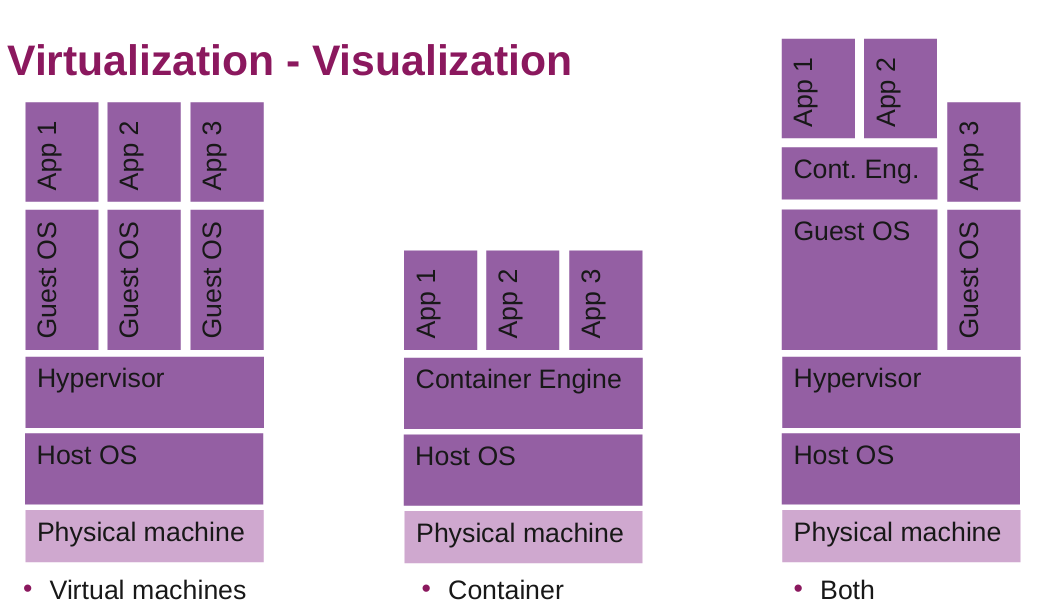
\includegraphics[width=0.75\linewidth]{Images/virtualization.png}
    \caption{Virtualization Overview}
\end{figure}

\subsection{Container}
\begin{itemize}
    \item Reduced size of Snapshots
    \item Quicker spinning up apps 
    \item Available memory ios shared
    \item Process-based isolation (shared kernel)
\end{itemize}

Technologies:
\begin{itemize}
    \item LXC (Linux Containers) - Lower abstraction level and direct use of Linux kernel features
    \item systemd-nspawn - Part of the systemd project, minimalist container manager
    \item Solaris Zones - Oracle/Sun-specific container technology
    \item Linux-VServer - Kernel patch for Linux, older virtualization technology
    \item OpenVz - Operating system-level virtualization, popular hosting tool
    \item rkt [ended]- CoreOS-developed alternative to Docker, focus on security
    \item Singularity - Scientifically oriented container solution, HPC-friendly
\end{itemize}

\subsubsection{Podman}
\begin{itemize}
    \item  Different architecture, docker runs a daemon and you connect via CLI, podman does not [source]
    \item Supports docker compose
\end{itemize}

\subsection{VM}
\begin{itemize}
    \item App can access all OS resources
    \item Live migrations
    \item Pre allocates memory
    \item Full isolation
    \item Better hardware utilization and resource sharing
\end{itemize}

\section{Loadbalancing}
Distribution of workloads across computing resources
with the options to:
\begin{itemize}
    \item Ensure HA and reliability
    \item Add or subtract server as demand dictates
\end{itemize}

\subsection{Types}
Types of LB:
\begin{enumerate}
    \item Hardware
    \item Cloud-Based
    \item Software
\end{enumerate}

Subtypes:
\begin{itemize}
    \item Layer 7 http
    \item DNS
        \begin{itemize}
            \item Round-Robin, very easy, static, caching with no fast changes
            \item Split Horizon DNS, different DNS per source of request
        \end{itemize}
    \item Layer 3 Anycast, needs AS, difficult, 
    
\end{itemize}

\subsection{Algorithms}
\begin{itemize}
    \item Round Robin, may drop req on congestion
    \item Weighted Round Robin, high variance in server load
    \item Least connections, latency issues
    \item Peak Exponentially weighted moving average, complexity
    \item Others: ip-hash, least-time, random, uri-hash, cookie
\end{itemize}

\section{Web Architectures}
\subsection{Server Side Rendering SSR}
In SSR the Server generates the resources.
User sends a request to the web server.
The server processes the request running server-side code.

The big advantage here is to use SEO.
Whereas the disadvantage os that it needs rendering for each request which
can be mitigated by generating a static site.
When using static site generators the site is generated when content changes.

\subsection{Single Page Application SPA}
In a SOA the client page updates as the user interacts with it.
It relies on JavaScript for dynamic behaviour.

One advantage is that the application does not require a page reload.
SEO only works if JS is executed at SE.

\subsection{CORS (Cross-Origin Resource Sharing)}
The browser restricts cross-origin requests from scripts.

Solution:
\begin{itemize}
    \item Reverse Proxy with builtin webserver
    \item Reverse Proxy with external webserver
    \item Modify CORS headers to include the correct domains
\end{itemize}

\defn{Hydration}{
    IN Hydration the first content is already presented in HTML, like in SSR.
    Further access howerer is then made via an API.
    So its the combination of SSR and SPA.
    
}

\section{Categorization}

\defn{Categorization}{
    \begin{description}
        \item[Tightly Coupled] processing elements, or nodes, have access to a common memory 
        \item[Loosely Coupled] No reference
    \end{description}
    \begin{itemize}
        \item Small-Scale (WebApp + Database)
        \item Large Scale
        \item Homogeneous
        \item Heterogeneous
        \item Decentraliced (not owned by one actor) vs Distributed
    \end{itemize}
}

\defn{CAP}{
    \begin{description}
        \item[Consistency] Every node has the same consistent state
        \item[Availability] Every non-failing node always returns a response
        \item[Partition Tolerant] The system continues to be consistent even when network partitions  
    \end{description}

    One can not guarantee all three.
}

\end{document}